\documentclass[11pt]{article}
\usepackage[a4paper, total={6in, 8.5in}]{geometry}
\usepackage[english]{babel}
\usepackage{graphicx}
\usepackage{hyperref}
\usepackage[onehalfspacing]{setspace}
\usepackage{float}
\usepackage{titlepic}
\usepackage{listings}
% \usepackage{xcolor}
\usepackage{amsmath}
\usepackage{amsfonts}
\usepackage{scrlayer-scrpage}
\usepackage{csquotes}
\usepackage{blkarray}
\usepackage{mwe}
\usepackage{algorithm}
\usepackage{algorithmic}
\usepackage{esvect}
\usepackage{physics}
\usepackage[table,xcdraw]{xcolor}


\usepackage[style=authoryear, backend=biber]{biblatex}
\usepackage{amssymb}
\addbibresource{references.bib}
\cfoot*{\pagemark}

\DeclareMathOperator*{\argmax}{arg\,max}
\DeclareMathOperator*{\argmin}{arg\,min}
\newcommand{\E}{\mathrm{E}}
\newcommand{\Var}{\mathrm{Var}}
\newcommand{\Cov}{\mathrm{Cov}}



\begin{document}
    \title{Autonomous Systems - Perception, Potential Fields}
    \date{06/2021}
    \author{Rupp Matthias}
    \maketitle
    \thispagestyle{empty}
    \vspace{2 cm}
    \begin{figure}[H]
        \centering
        
\includegraphics[width = 6cm]{Logo-A3}\label{fig:logo}
    \end{figure}
    \pagebreak

    \ohead{Rupp Matthias}
    \tableofcontents
    \thispagestyle{empty}
    \clearpage

    \definecolor{codegreen}{rgb}{0,0.6,0}
    \definecolor{codegray}{rgb}{0.5,0.5,0.5}
    \definecolor{codepurple}{rgb}{0.58,0,0.82}
    \definecolor{backcolour}{rgb}{0.95,0.95,0.92}

    \lstdefinestyle{mystyle}{
        backgroundcolor=\color{backcolour},
        commentstyle=\color{codegreen},
        keywordstyle=\color{magenta},
        numberstyle=\tiny\color{codegray},
        stringstyle=\color{codepurple},
        basicstyle=\ttfamily\footnotesize,
        breakatwhitespace=false,
        breaklines=true,
        captionpos=b,
        keepspaces=true,
        numbers=left,
        numbersep=5pt,
        showspaces=false,
        showstringspaces=false,
        showtabs=false,
        tabsize=2
    }
    \lstset{style=mystyle}

    \section{Attracting field}\label{sec:attracting-field}
    The first important part of the potential field is the attracting potential of the goal.
    \autoref{eq:uatt} shows the formula to calculate said attracting potential.
    \begin{equation}\label{eq:uatt}
        U_{a t t}(q)=\frac{1}{2} k_{a t t} \cdot \rho_{\text {goal }}^{2}(q)
    \end{equation}
    Where $k_{a t t }$ is a scaling factor, while $\rho_{\text {goal }}$ is the euclidean distance from the current position in the field to the goal.
    The resulting field for the parameters given in the task description can be seen in \autoref{fig:attfield}.
    \begin{figure}[H]
        \centering
        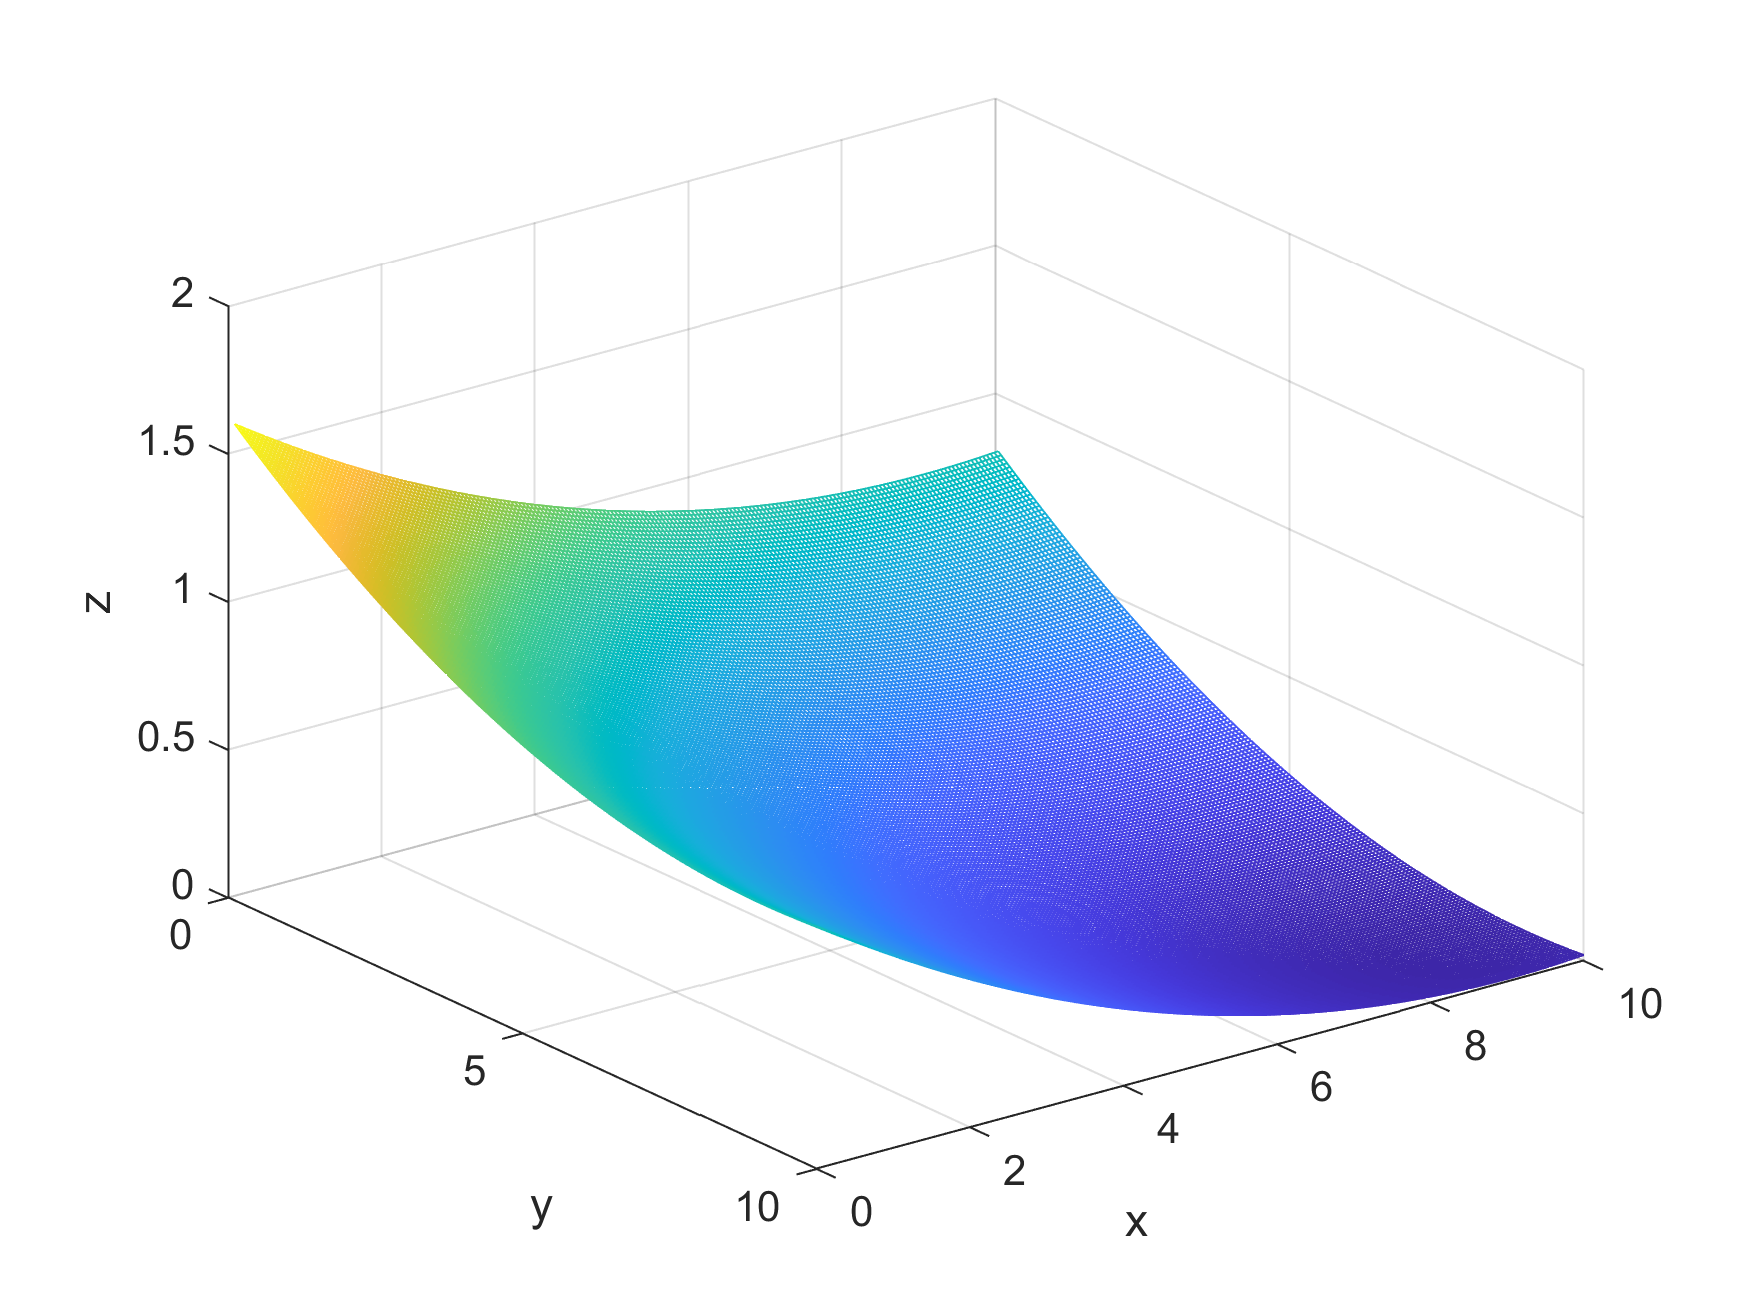
\includegraphics[width=1.0\textwidth]{../test/images/u_att}
        \caption{Attracting field}
        \label{fig:attfield}
    \end{figure}
    As can be seen, the resulting field resembles a slope that "drops" into the goal.
    When placing a robot at a random point in the field, it will "roll" into the goal due to the slope (the gradient).
    This is the effect of the attracting potential field.

    \section{Repelling field}\label{sec:rep-field}
    The second part of the potential field is the repelling potential of the obstacles.
    Said repelling potential should be very strong when close to the obstacle, but have no influnce when the robot is further away from the obstacle.
    A formula for said potential can be seen in \autoref{eq:urep}.
    \begin{equation}\label{eq:urep}
        U_{\text {rep }}(q)=\left\{\begin{array}{ll}
                                       \frac{1}{2} k_{\text {rep }}\left(\frac{1}{\rho(q)}-\frac{1}{\rho_{0}}\right)^{2} & \text { for } \rho(q)<\rho_{0} \\
                                       0 & \text { for } \rho(q) \geq \rho_{0}
        \end{array}\right.
    \end{equation}
    $k_{\text {rep }}$ is a scaling factor, $\rho(q)$ is the minimal distance of the robot to the obstacle at position $q$.
    $\rho_{0}$ is distance to which the obstacle influences the robot.
    This way, the condition for the repelling potential having no influence when the robot is far away from the obstacle, but being strong when close to an obstacle is fulfilled.
    Plotting the repelling field with the parameters from the task sheet and the given formula results in \autoref{fig:repfield}.
    \begin{figure}[H]
        \centering
        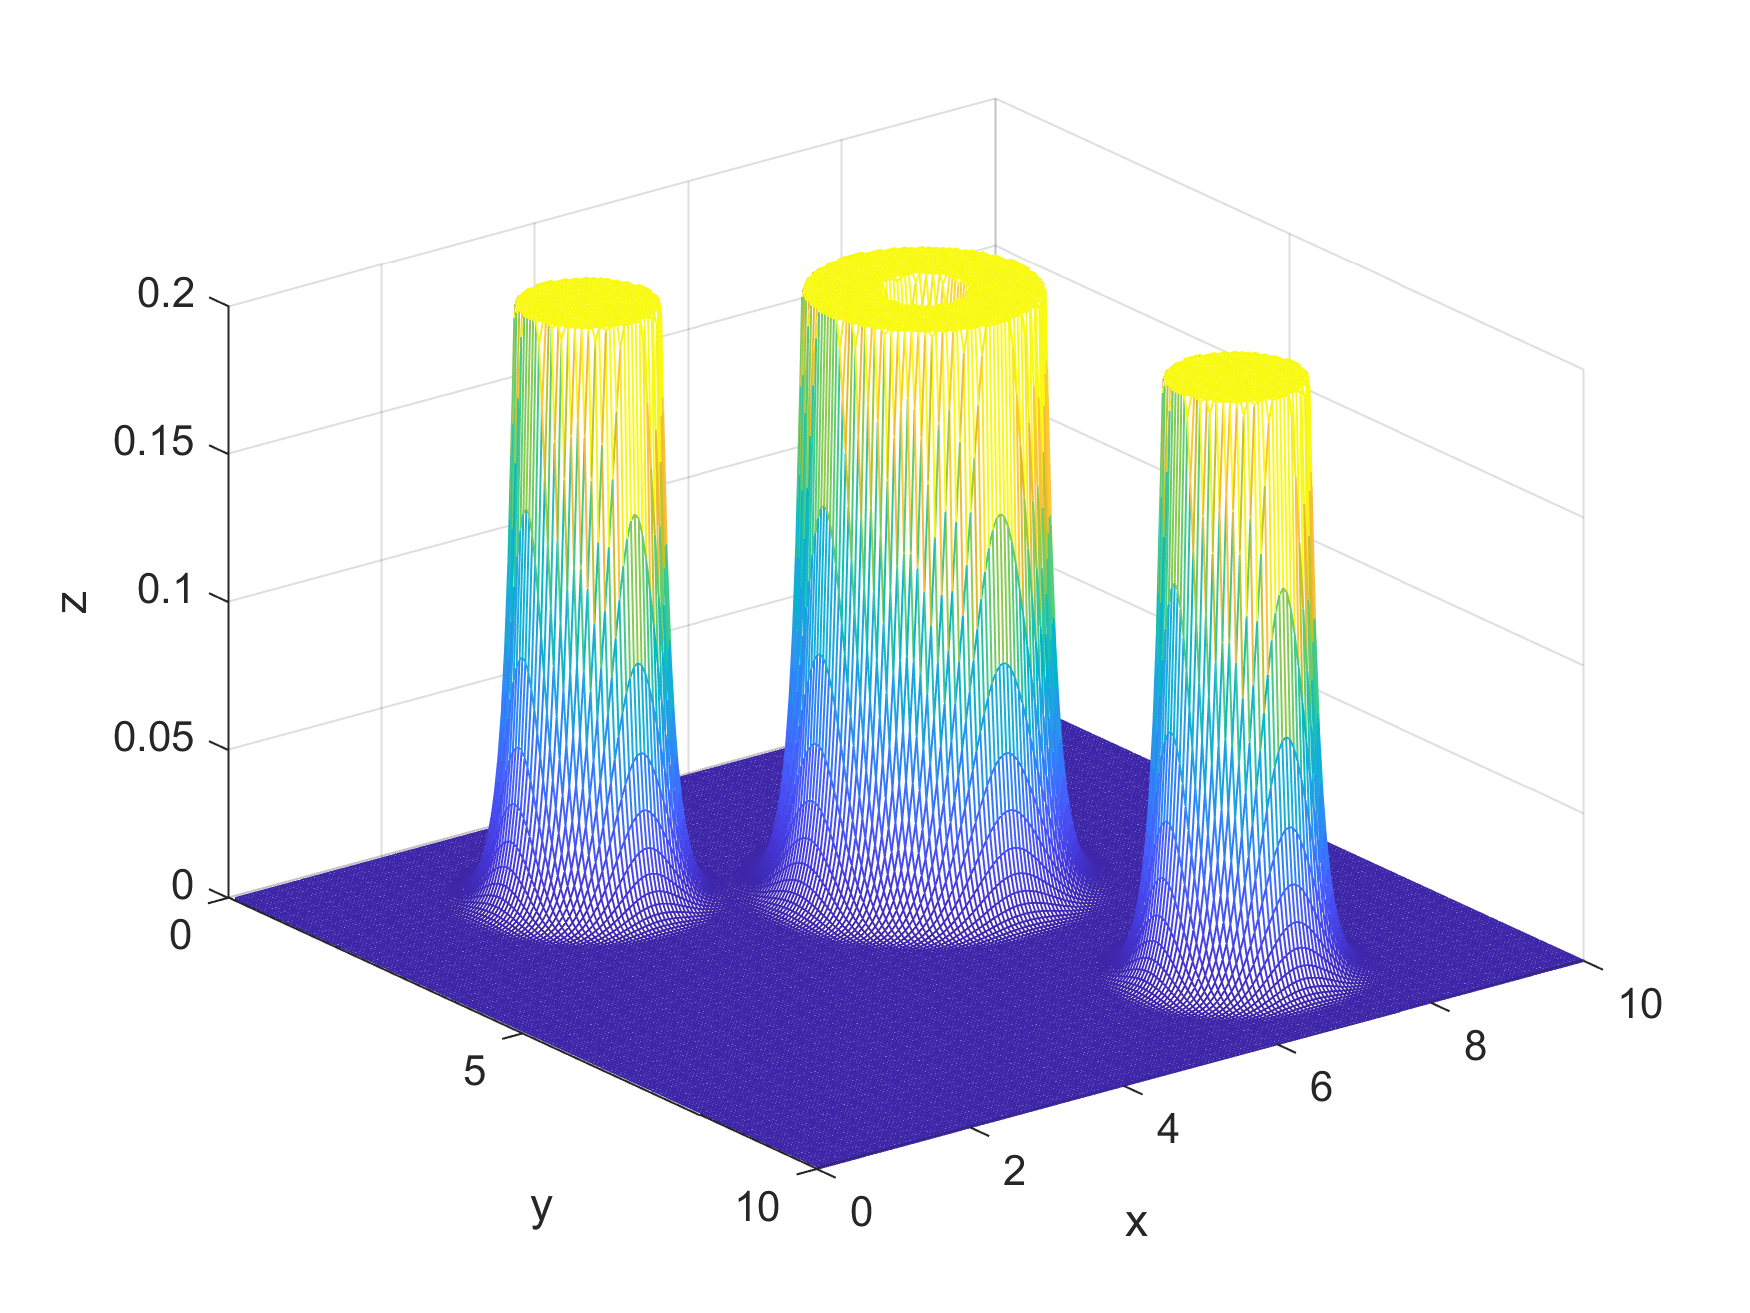
\includegraphics[width=1.0\textwidth]{../test/images/u_rep}
        \caption{Repelling field}
        \label{fig:repfield}
    \end{figure}
    The field is flat everywhere but where the obstacles are located, where the repelling force becomes very large.
    Note that the repelling potential has been limited to a certain height for a prettier plot.

    \section{Total potential field}\label{sec:totfield}
    The final step to get the potential field is to combine the attracting and repelling potentials.
    This can be done with the simple \autoref{eq:totalfield}.
    \begin{equation}\label{eq:totalfield}
        U(q)=U_{a t t}(q)+U_{r e p}(q)
    \end{equation}
    As can be seen, this is simply a combination of the attracting and repelling potentials.
    This will yield \autoref{fig:potfield}.
    \begin{figure}[H]
        \centering
        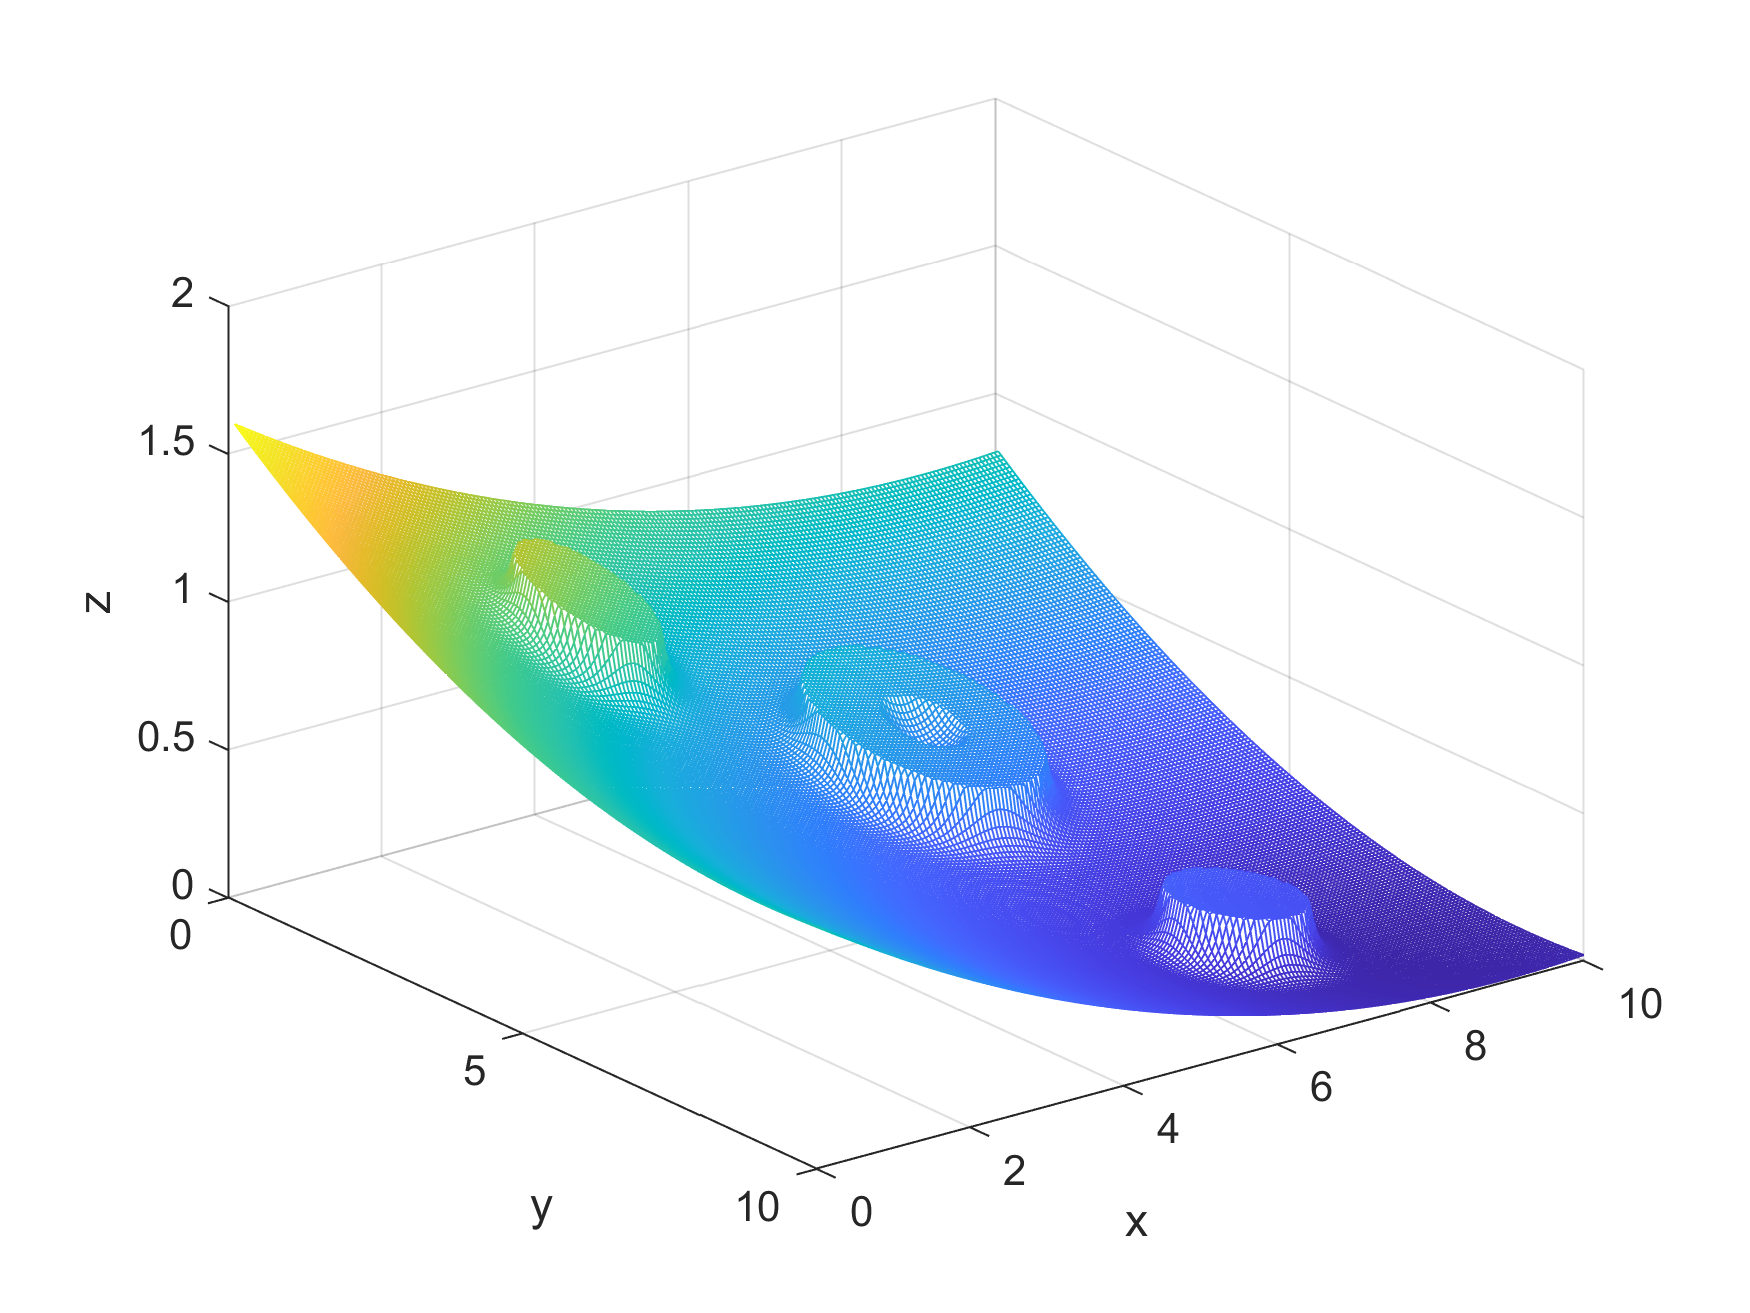
\includegraphics[width=1.0\textwidth]{../test/images/u_combi}
        \caption{Total potential field}
        \label{fig:potfield}
    \end{figure}
    This is clearly a combination of \autoref{fig:attfield} and \autoref{fig:repfield}.
    With this potential field, the robot will "roll" towards the goal due to the attracting potential, while the repelling force close to the obstacles will push it around them, while still heading towards the goal due to the attracting potential.

    \section{Forces in the potential field}\label{sec:forcesinfield}
    The potential field exerts forces on the robot placed in it, which will cause the robot to move towards the goal along a path.
    The total force exerted on the robot can be calculated with \autoref{eq:ftot}.
    \begin{equation}\label{eq:ftot}
        F(q)=F_{a t t}(q)+F_{r e p}(q)=-\nabla U_{a t t}(q)-\nabla U_{r e p}(q)
    \end{equation}
    Once again, this is a combination of attracting and repelling forces.
    The attracting force can be calculated with \autoref{eq:fatteq}.
    \begin{equation}\label{eq:fatteq}
        F_{a t t}(q)=-\nabla U_{a t t}(q)=-k_{a t t} \cdot \rho_{g o a l}(q) \nabla \rho_{g o a l}(q)=-k_{a t t} \cdot\left(q-q_{g o a l}\right)
    \end{equation}
    The repelling force can be calculated with \autoref{eq:frepeq}.
    \begin{equation}\label{eq:frepeq}
        F_{\text {rep }}(q)=-\nabla U_{\text {rep }}(q)=\left\{\begin{array}{ll}
                                                                   k_{\text {rep }}\left(\frac{1}{\rho(q)}-\frac{1}{\rho_{0}}\right) \frac{q-q_{0}}{\rho^{3}(q)} & \text { for } \rho(q)<\rho_{0} \\
                                                                   0 & \text { for } \rho(q) \geq \rho_{0}
        \end{array}\right.
    \end{equation}
    To calculate the robot path based on these formulas, the robot is placed at a starting postion.
    Note that the goal position also need to be known from the beginning.
    From this starting position, the attracting and repelling forces are calculated.
    Said forces are vectors, in our concrete examples, so the new position is calculated by adding the attracting and repelling force vectors to the robot position.
    Based on this new robot position, this process is repeated, until the goal is reached.
    Using a starting position of $\left( 2, 1 \right)$ and a goal position of $\left( 9, 9 \right)$, the robot will take the path seen in \autoref{fig:robpath}, based on the potential field seen in \autoref{fig:potfield}.
    \begin{figure}[H]
        \centering
        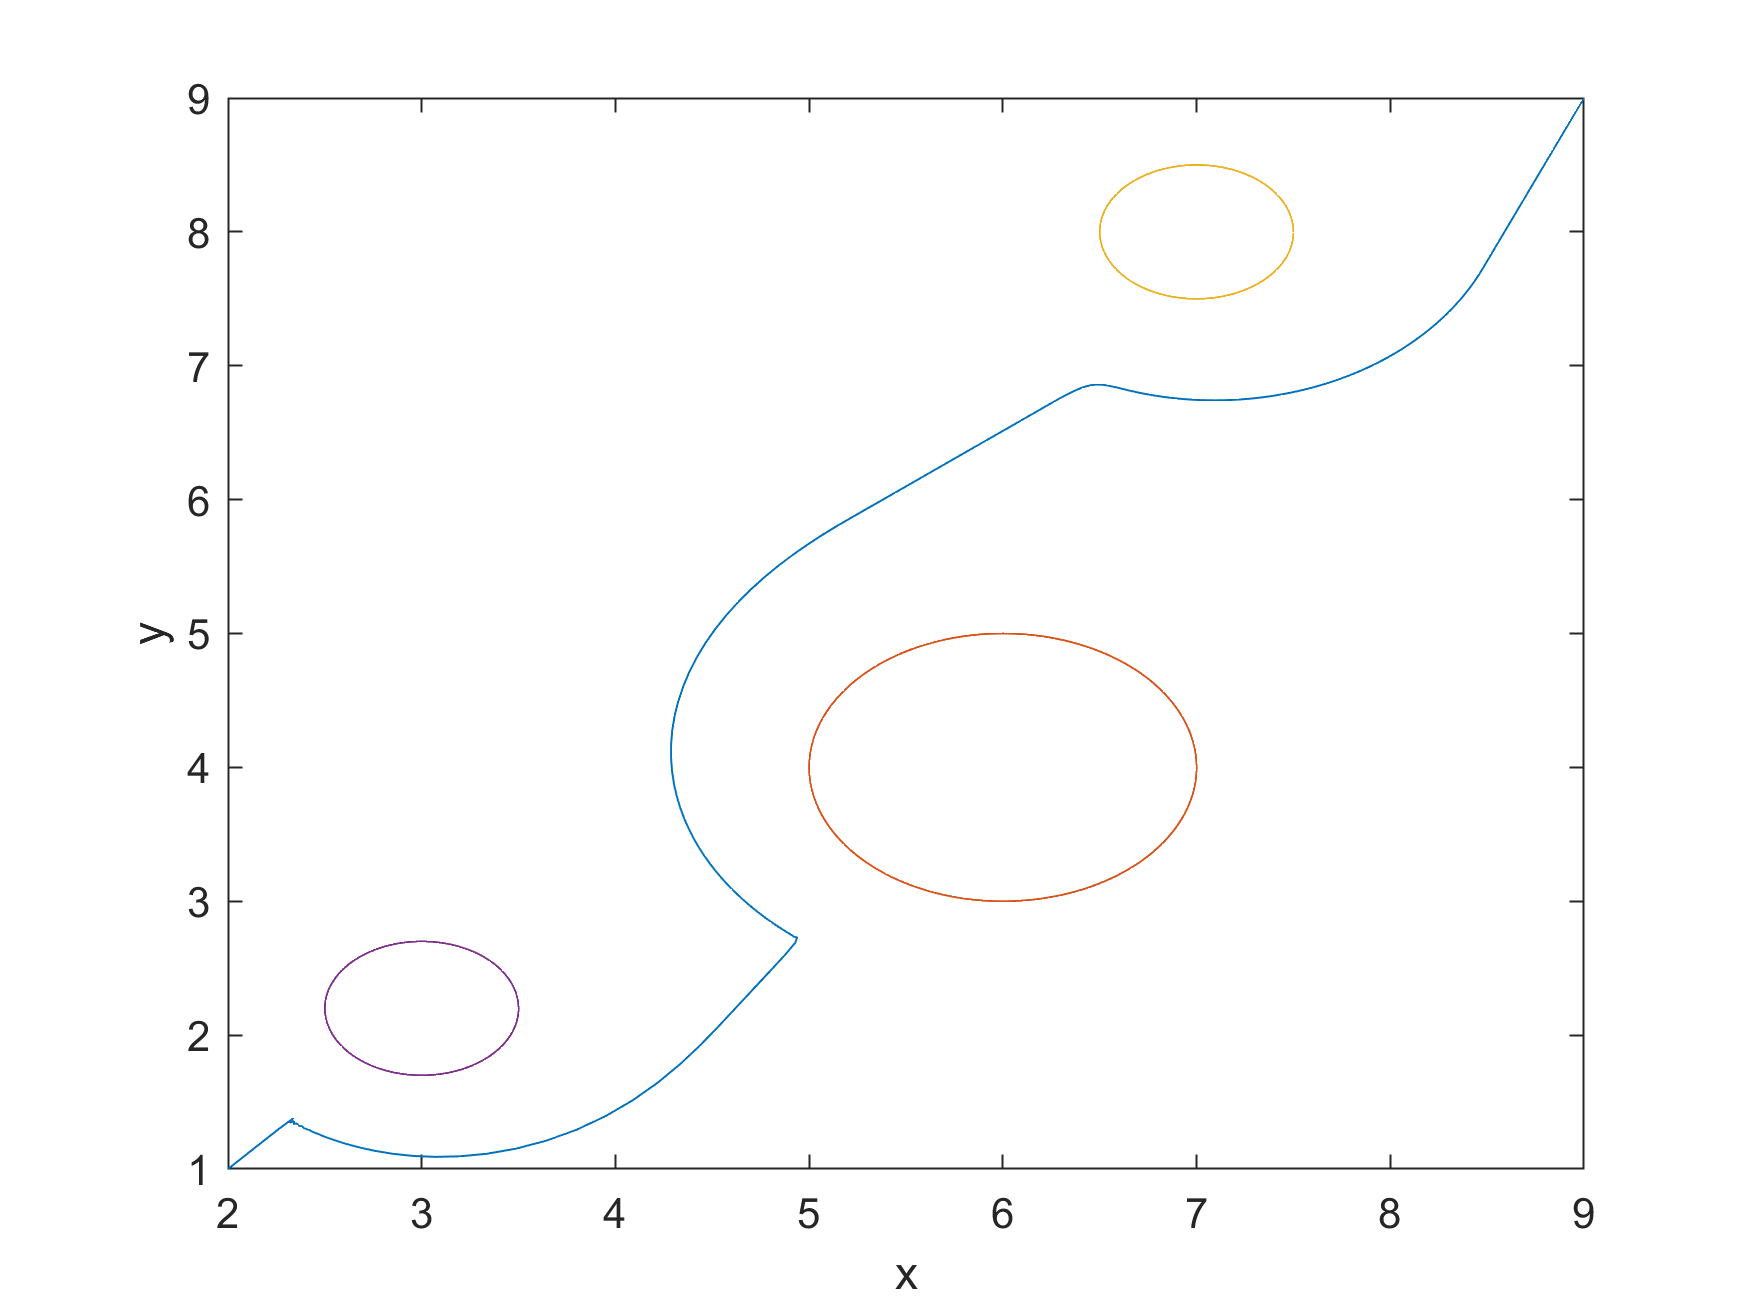
\includegraphics[width=1.0\textwidth]{../test/images/robot_path}
        \caption{Robot path through potential field}
        \label{fig:robpath}
    \end{figure}
    The circles represent the obstacles, the red cross is the starting position, the green cross is the goal position.
    The blue line is the path the robot takes due to the potential field.\newline
    The robot moves towards the goal, until coming close enough to an obstacle that the repelling potential influences the path.
    The repelling potential of the obstacle, combined with the attracting potential of the goal, pushes the robot around the obstacle.
    After leaving the distance where the repelling force is effective, the attracting force is now the sole factor influencing the robot again, and it heads directly towards the goal again.
    Said process repeats until the robot has reached the goal.

    \clearpage
    \phantomsection
    \addcontentsline{toc}{section}{References}
    \printbibliography

    \clearpage
    \phantomsection
    \addcontentsline{toc}{section}{List Of Figures}
    \listoffigures


\end{document}